\section{Работа. Закон сохранения энергии}

\introProblems

\begin{ex} %Сив162
Коэффициент трения между некоторым телом и плоскостью, наклоненной под углом $45^{\circ}$ к горизонту, равен 0,2. На какую высоту поднимается это тело, скользя по наклонной плоскости, если ему будет сообщена скорость 10 м/с, направленная вверх вдоль плоскости? Какова будет скорость тела, когда оно вернется в нижнюю исходную точку своего движения?
\begin{ans}
4,25 м; $\approx$ 8,16 м/с.
\end{ans}
\end{ex}

\begin{ex} %Сив166
Из залитого подвала, площадь пола которого равна 50 м\textsuperscript{2}, требуется выкачать воду на мостовую. Глубина воды в подвале 1,5 м, а расстояние от уровня воды в подвале до мостовой 5 м. Найти работу, которую необходимо затратить для откачки воды.
\begin{ans}
4,3 МДж.
\end{ans}
\end{ex}

\begin{ex} %Сив170
Определить среднюю полезную мощность при выстреле из гладкоствольного ружья, если известно, что пуля массы $m$ вылетает из ствола со скоростью $v_0$, а длина канала ствола $l$ (давление пороховых газов считать постоянным во все время нахождения снаряда в канале ствола).
\begin{ans}
$N =\frac{mv_{0}^3}{4l}$.
\end{ans}
\end{ex}


\begin{ex} %Сив196
На гладком горизонтальном столе лежит шар массы $m_1$, соединенный с пружиной жесткости $k$. Второй конец пружины закреплен (рис. \ref{2BallsSpring}). Происходит лобовое упругое соударение этого шара с другим шаром, масса которого $m_2$ меньше $m_1$, а скорость равна $v$. В какую сторону будет двигаться второй шар после удара? Определить амплитуду колебаний первого шара после соударения.

\begin{figure}[h]
\centering
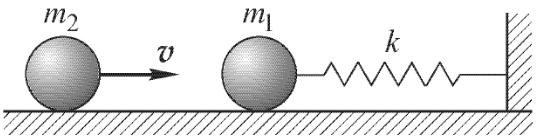
\includegraphics[width=0.5\textwidth]{2BallsSpring.png}
\caption{}
\label{2BallsSpring}
\end{figure}

\begin{ans}
После соударения второй шарик отскочит назад, $A = \frac{2m_2v}{m_1+m_2}\sqrt{\frac{m_1}{k}}$.
\end{ans}
\end{ex}

\begin{ex} %Сив227
Баллистический маятник — это маятник, употребляющийся для определения скорости снаряда. Принцип его действия заключается в том, что снаряд, скорость которого следует измерить, ударяется в тело маятника длины $l$ (рис. \ref{ballisticPendulum}). Если известны условия удара и массы снаряда $m$ и маятника $M$, то по углу отклонения маятника $\alpha$ можно вычислить скорость $v$ снаряда до удара. Показать, как это сделать для случая, когда снаряд после удара застревает в маятнике.

\begin{figure}[h]
\centering
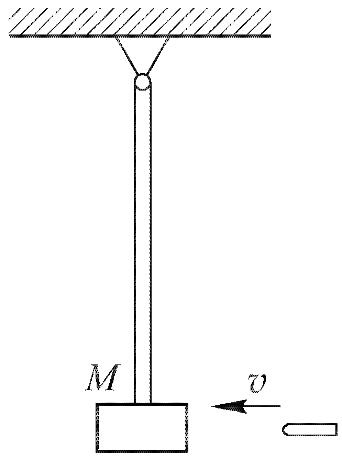
\includegraphics[width=0.25\textwidth]{ballisticPendulum.png}
\caption{}
\label{ballisticPendulum}
\end{figure}

\begin{ans}
$v = 2\frac{M+m}{m}\sqrt{lg}\sin \frac{\alpha}{2}$.
\end{ans}
\end{ex}

\qualProblems

\begin{ex}
Знак многих физических величин зависит от выбора системы координат, например, проекция ускорение сводного падения может быть положительной, если ось направить вниз, или отрицательной, если ось направить вверх. Может ли механическая работа подобным образом изменять знак в разных системах координат?
\end{ex}

\begin{ex}
Какая из следующих сил ни при каких обстоятельствах не совершает работу:
\begin{itemize}
\item гравитационная сила;
\item сила трения покоя;
\item сила трения скольжения;
\item сила натяжения;
\item сила реакции опоры.
\end{itemize}
\end{ex}

\begin{ex}
Эскалатор движется вниз с постоянной скорость. Вы поднимаетесь по эскалатору с такой же скоростью вверх, таким образом относительно земли остаетесь на месте. Совершаете ли Вы работу при этом?
\end{ex}

\begin{ex}
Веревку, привязанную к телу, тянут с постоянной силой, заставляя тело двигаться с постоянным ускорением. Согласно 3 закону Ньютона, тело действует на веревку с такой же по модулю силой в противоположном направлении. Будет ли суммарная работа этих сил равна нулю? Если да, то за счет какой работы увеличивается кинетическая энергия тела? 
\end{ex}

\begin{ex}
За счет изменения какой энергии воздушный шар поднимается вверх?
\end{ex}

\begin{ex}
Тело бросают под углом к горизонту под различными углами с одинаковой начальной скорость. Начальная кинетическая энергия во всех случаях одинакова, почему же различна высота подъема (максимальная потенциальная энергия)?
\end{ex}

\begin{ex}
Человек прыгает на батуте, при этом с каждым прыжком его максимальная высота подъема (потенциальная энергия) увеличивается. Трение о воздух, наоборот, должно приводить к уменьшению механической энергии системы. За счет чего растет энергия системы?
\end{ex}

\begin{ex}
Изобразите график зависимости потенциальной энергии гравитационного взаимодействия Земли и тела вблизи ее поверхности. Как использовать этот график для объяснения свободного тел на Землю?
\end{ex}

\begin{ex}
Может ли действие силы трения привести к увеличение механической энергии системы? Если да, приведите примеры. 
\end{ex}

\simpleProblems

\begin{ex} %Сив163
Какую работу надо совершить, чтобы втащить (волоком) тело массы $m$ на горку с длиной основания $L$ и высотой $H$, если коэффициент трения между телом и поверхностью горки равен $\mu$? Как изменится ответ, если угол наклона поверхности горки с горизонтом может меняться вдоль горки, но его знак остается постоянным.
\begin{ans}
$A=mg(H+\mu L)$.
\end{ans}
\end{ex}

\begin{ex}
Оконная штора массой в 1 кг и длиной 2 м свертывается на тонкий валик наверху окна. Какая при этом совершается работа? Трением пренебречь.
\begin{ans}
$A \approx 10$ Дж.
\end{ans}
\end{ex}

\begin{ex} %Сив176
Какую мощность $N$ затрачивает лошадь на движение саней, если она тянет их в гору равномерно со скоростью $v$? Масса саней $m$ и трение между санями и поверхностью горы постоянно, коэффициент трения $\mu$. Угол наклона горы $\alpha$.
\begin{ans}
$N = mgv(\mu \cos \alpha +\sin \alpha)$.
\end{ans}
\end{ex}

\begin{ex} %МФТИ4.8
Шайба массы $m$, скользя по льду, сталкивается с неподвижной шайбой массы $3m$. Считая удар упругим и центральным, определить, на какое расстояние $S$ разлетятся шайбы, если скорость первой шайбы перед ударом была $v$, а коэффициент трения между шайбами и льдом равен $\mu$.
\begin{ans}
$S = \frac{v^2}{4 \mu g}$.
\end{ans}
\end{ex}

\begin{ex} %МФТИ4.2
Математический маятник длиной $l$ находится в положении равновесия. Определите, какую скорость $u$ надо сообщить грузу, чтобы он мог совершить полный оборот, для двух случаев: груз подвешен а) на жестком стержне и б) на нерастяжимой нити.
\begin{ans}
$v_1 = 2\sqrt{gl}$, $v_2 = \sqrt{5gl}$.
\end{ans}
\end{ex}

\begin{ex} %Сив179
Определить отношение потенциальных энергий деформации $U_1$ и $U_2$ двух пружин с коэффициентами упругости $k_1$ и $k_2$ в двух случаях: 1) пружины соединены последовательно и растягиваются грузом $Р$ (рис. \ref{2Springs}а); 2) пружины висят параллельно, причем груз $Р$ подвешен в такой точке, что обе пружины растягиваются на одну и ту же величину (рис. \ref{2Springs}б). Деформацией пружин под действием собственного веса пренебречь.

\begin{figure}[h]
\centering
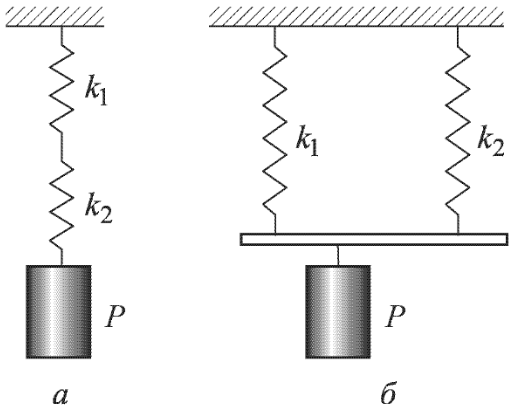
\includegraphics[width=0.5\textwidth]{2Springs.png}
\caption{}
\label{2Springs}
\end{figure}

\begin{ans}
1) $U_1/U_2 = k_2/k_1$; 2) $U_1/U_2 = k_1/k_2$.
\end{ans}
\end{ex}

\complexProblems

\begin{ex} %Сив197
Система состоит из двух шариков с массами $m$ и $M$, соединенных между собой невесомой пружиной с коэффициентом жесткости $k$ (рис. \ref{3BallsSpring}). Третий шарик с массой $m$, движущийся вдоль оси пружины со скоростью $v$, претерпевает упругое столкновение с шариком $m$, как указано на рис. \ref{3BallsSpring}. Считая шарики абсолютно жесткими, найти после столкновения: 1) кинетическую энергию $K$ движения системы как целого; 2) внутреннюю энергию системы $E_1$; 3) амплитуду колебаний одного шарика относительно другого $A$. До удара система покоилась, а пружина не была деформирована. Какие шарики могут рассматриваться как абсолютно жесткие?	

\begin{figure}[h]
\centering
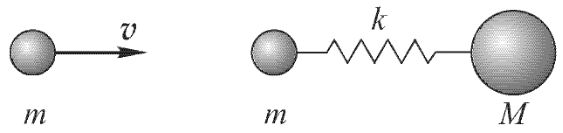
\includegraphics[width=0.5\textwidth]{3BallsSpring.png}
\caption{}
\label{3BallsSpring}
\end{figure}

\begin{ans}
1) $K=\frac{m^2v^2}{2(M+m)}$; 2) $E_1 = \frac{Mmv^2}{2(M+m)}$; 3) $A = v\sqrt{\frac{Mm}{k(M+m)}}$.
\end{ans}
\end{ex}

\begin{ex}  %Сив232
От поезда, идущего с постоянной скоростью, отрывается последний вагон, который проходит путь $l$ и останавливается. На каком расстоянии от вагона в момент его остановки будет находиться поезд, если тяга паровоза постоянна, а трение каждой части поезда не зависит от скорости и пропорционально ее весу? Масса поезда до момента отрыва вагона $M$, масса вагона $m$.
\begin{ans}
$x = Ml/(M-m)$.
\end{ans}
\end{ex}

\begin{ex} %Сив229
Два маятника в виде шариков разных масс $m_1$ и $m_2$ свободно подвешены на нитях разной длины $l_1$ и $l_2$ так, что шарики соприкасаются. Первый маятник отводят в плоскости нитей на угол $\alpha$ от первоначального положения и отпускают. Происходит центральный удар шариков. На какие углы $\alpha_1$ и $\alpha_2$ относительно отвесной линии отклонятся маятники после удара (углы считать малыми, удар считать упругим)?
\begin{ans}
$\alpha_1 =\frac{m_1-m_2}{m_1+m_2}\alpha$, $\alpha_2 =\frac{2m_1}{m_1+m_2}\alpha \sqrt{\frac{l_1}{l_2}}$.
\end{ans}
\end{ex}

\begin{ex} %Чертов2.69
Камешек скользит с наивысшей точки купола, имеющей форму полусферы. Какую дугу $\alpha$ опишет камушек, прежде чем оторвется от поверхности купола? Трением пренебречь.
\begin{ans}
$\alpha = \arccos(2/3)$.
\end{ans}
\end{ex}

\clearpage